\documentclass[oneside]{book}% openany
\usepackage[utf8]{inputenc}
\usepackage[T1]{fontenc}
\usepackage[french]{babel}
\usepackage{booktabs}
\usepackage{tabularx}
\usepackage{mathpazo}
\usepackage{epigraph}
\usepackage{graphicx}
\usepackage{pdfpages}
\usepackage{here}
\usepackage{array}
\usepackage{hyperref}
\hypersetup{
    colorlinks=true,
    linkcolor=blue,
    filecolor=magenta,      
    urlcolor=cyan,
    pdftitle={Overleaf Example},
    pdfpagemode=FullScreen,
    }

\usepackage{tcolorbox}
\tcbuselibrary{skins, minted, breakable, listings}

\newtcblisting{mycpp}{breakable, enhanced, listing engine=minted,
minted style=colorful,
minted language=C++,
minted options={fontsize=\footnotesize,breaklines,autogobble,linenos,numbersep=3mm},
colback=blue!5!white,colframe=blue!75!black,listing only,
left=5mm,enhanced,
overlay={\begin{tcbclipinterior}\fill[red!20!blue!20!white] (frame.south west)
rectangle ([xshift=5mm]frame.north west);\end{tcbclipinterior}}}

\newtcblisting{commandshell}{colback=black,colupper=white,colframe=yellow!75!black, listing only,listing options={style=tcblatex,language=sh}, breakable, enhanced}


\begin{document}
  %----------------------------------------------------------------------------------------
%	TITLE PAGE
%----------------------------------------------------------------------------------------

\begin{titlepage} % Suppresses displaying the page number on the title page and the subsequent page counts as page 1
	\newcommand{\HRule}{\rule{\linewidth}{0.5mm}} % Defines a new command for horizontal lines, change thickness here
	
	\center % Centre everything on the page
	
	%------------------------------------------------
	%	Headings
	%------------------------------------------------
	
	\textsc{\LARGE Université Virtuelle de Tunis}\\[1.5cm] % Main heading such as the name of your university/college
	
	\textsc{\Large Master IASRIA}\\[0.5cm] % Major heading such as course name
	
	\textsc{\large Mini-projet Electronique}\\[0.5cm] % Minor heading such as course title
	
	%------------------------------------------------
	%	Title
	%------------------------------------------------
	
	\HRule\\[0.4cm]
	
	{\huge\bfseries Détection des troubles cardiologiques à partir de l'analyse des ECG}\\[0.4cm] % Title of your document
	
	\HRule\\[1.5cm]
	
	%------------------------------------------------
	%	Author(s)
	%------------------------------------------------
	
	\begin{minipage}{0.4\textwidth}
		\begin{flushleft}
			\large
			\textit{Auteurs}\\
			R. \textsc{ALOUI}\\ % Your name
			N. \textsc{AZZOUZ}\\ % Your name
			A. \textsc{MALLEH} % Your name
		\end{flushleft}
	\end{minipage}
	~
	\begin{minipage}{0.4\textwidth}
		\begin{flushright}
			\large
			\textit{Directeur}\\
			Dr. Farah \textsc{CHANCHEH} % Supervisor's name
		\end{flushright}
	\end{minipage}
	
	% If you don't want a supervisor, uncomment the two lines below and comment the code above
	%{\large\textit{Author}}\\
	%John \textsc{Smith} % Your name
	
	%------------------------------------------------
	%	Date
	%------------------------------------------------
	
	\vfill\vfill\vfill % Position the date 3/4 down the remaining page
	
	{\large\today} % Date, change the \today to a set date if you want to be precise
	
	%------------------------------------------------
	%	Logo
	%------------------------------------------------
	
	%\vfill\vfill
	%\includegraphics[width=0.2\textwidth]{placeholder.jpg}\\[1cm] % Include a department/university logo - this will require the graphicx package
	 
	%----------------------------------------------------------------------------------------
	
	\vfill % Push the date up 1/4 of the remaining page
	
\end{titlepage}

  \frontmatter
  %\tableofcontents
  \chapter*{Remerciements}

\vspace*{3cm}
\epigraph{Si j'ai pu voir plus loin, c'est que je me tenais sur les épaules de géants.}{\textit{Isaac Newton}}

Nous tenons à exprimer toutes notre reconnaissance envers nos enseignants. Pour le sérieux, l'engagement et l'encadrement de M. {\bf Rached GHARBI}, nous sommes fiers de passer sous votre direction.
  \mainmatter
  \chapter*{Introduction générale}
\addcontentsline{toc}{chapter}{Introduction générale}
Les variétés de l'activité humaine aujourd'hui exige le suivi de l'état de santé à proximité. Ce qui s'est traduit par l'augmentation des équipements portés (wearable healthcare) de suivi du santé chaque année par 24\% chaque année\footnote{https://www.insiderintelligence.com/insights/wearable-technology-healthcare-medical-devices/} \cite{3}. La montre intélligente offre plusieurs services outre que le temps. La diversité de ces équipements prend plusieurs formes et assure la collecte de plusieurs métriques, la pression artérielle, concentration de $O_2$, \ldots

L'électrocardiogramme (ECG) est un test simple pour se renseigner rapidement sur le rythme et l'activité électrique du c\oe ur. C'est pourquoi l'analyse d'une telle information critique aide à conclure sur la normalité de l'activité cardiaque d'une façon générale. L'analyse du signal ECG, selon le type d'analyse, peut se faire sur plusieurs étapes, le traitement du signal, l'extraction des caractéristiques, les transformations et finalement la classification \cite{1, 2}.

Aujourd'hui, la connectivité peut améliorer l'acquisition et l'enregistrement des données. C'est l'ère des objets connectés où ces objets peuvent envoyer les informatios sur des plateformes dédiées. Ces plateformes offrent d'autres traitements sur les données collectées.

Nous voulons, dans ce projet, concevoir un système de suivi de l'activité cardiaque. La solution doit être connectée. Le présent rapport détaille les étapes de conception et de réalisation de la solution.
  \chapter{Description de la solution}
\section{Mise en cadre du projet\label{cahiercharges}}
Rappelons que la solution doit :
\begin{enumerate}
  \item assurer suivi de l'activité cardiaque,
  \item effectuer sauvegarde des différentes valeurs,
  \item la base de donnée doit être accessible via le web.
\end{enumerate}
\section{Composante matérielle}
En se basant sur les recommendations de la section \ref{cahiercharges}, la selection des équippements peut être raffinée. Comment peut effectuer le suivi de l'activité cardiaque? l'un des capteur permettant une telle opération est le capteur AD8232. La section suivante donne plus de détails.
\subsection{Le capteur AD8232 \label{sec:capteurAD8232}}
Le module AD8232 assure la surveillance des impulsions cardiaque. Le kit apporte en plus 3 électrodes à placer sur le corp du patient. Ce module, dont le datasheet est disponible sur ce \href{https://www.analog.com/media/en/technical-documentation/data-sheets/ad8232.pdf}{lien} (voir Annexe \ref{Datasheet}), est caractérisé principalement par :
\begin{itemize}
  \item un filtre passe-haut à deux pôles pour éliminer les artefacts de mouvement et le potentiel de demi-cellule d'électrode
  \item un amplificateur opérationnel sans contrainte pour construire un filtre passe-bas à trois pôles éliminant les bruits suplémentaires
  \item température nominale de $[0;70]$ et de travail $[-40; 85]$
  \item alimentation faible de 3,3V
  \item il est conçu pour extraire, amplifier et filtrer les petits signaux bipotentiels en présence de conditions bruyantes.
\end{itemize}

\begin{figure}[H]
  \centering
  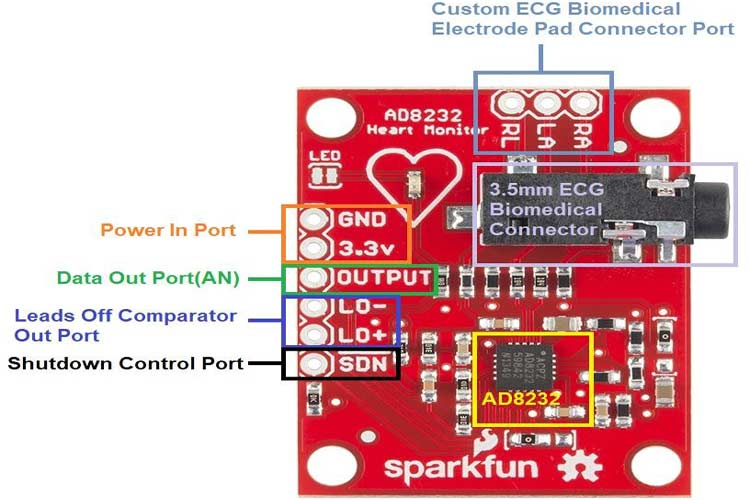
\includegraphics[scale=.4]{imgs/AD8232-Module-Overview.jpg}
  \caption{Description du capteur AD8232}
\end{figure}

Le tableau \ref{table:AD8232PINOUT} donne les pins du capteur
\begin{table}[H]
  \centering\small
  \begin{tabular}{lp{0.6\textwidth}}
  \toprule
  {\bf PIN}&{\bf Description}\\
  \toprule
  \mintinline{c++}{GND}&la masse\\
  \midrule
  \mintinline{c++}{3.3V}&alimentation\\
  \midrule
  \mintinline{c++}{Output} (ADC)&la sortie traitée du signal\\
  \midrule
  \mintinline{c++}{LO-}&leads off detection mode. \mintinline{c++}{LO-} est \mintinline{c++}{HIGH} si l'électrode rouge est déconnectée, et \mintinline{c++}{LOW} sinon\\
  \midrule
  \mintinline{c++}{LO+}&leads off detection mode. \mintinline{c++}{LO+} est \mintinline{c++}{HIGH} si l'électrode jaune est déconnectée, et \mintinline{c++}{LOW} sinon\\
  \midrule
  \mintinline{c++}{SDN}&Shutdown Control Input. Si cette pin est \mintinline{c++}{LOW}, le capteur active le mode de faible consommation\\
  \bottomrule
  \end{tabular}
  \caption{AD8232 PINOUT}
  \label{table:AD8232PINOUT}
\end{table}
\subsection{Carte de développement}
La section \ref{sec:capteurAD8232} a détaillé les carectéristiques techniques du capteur. Maintenant, une foi le capteur délivre l'activité électrique via sa pin \mintinline{c++}{Output}, vers quelle carte de développement cette information sera finalement acheminée ?

Pour répondre à cette question, il est recommander de revoir les recommendations citées dans la section \ref{cahiercharges}. En effet, l'activité cardiaque doit être envoyée vers le WEB. Ce qui impose que la carte doit pouvoir se connecter à INTERNET. Une recherche comparative entre les différents boards éligibles tels que Arduino (avec ses variantes), STM32, ESP32 \ldots a été établie. Les critères de sélection retenus sont la connectivité, le prix et la disponibilité. Finalement, la carte ESP32 est celle qui répond mieux aux différentes contraintes. Elle offre plusieurs types de connectivités (WIFI, Bluetooth) avec un prix minimal.


\begin{figure}[H]
  \centering
  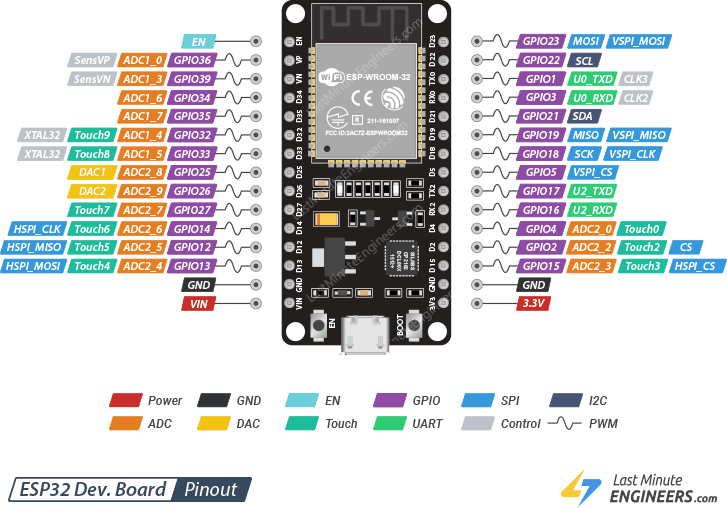
\includegraphics[scale=2]{imgs/ESP32-Pinout.png}
  \caption{Description de la carte de développement ESP32}
\end{figure}

L'ESP32 est un microcontroleur dont le constructeur est \textit{Espressif}. Ce constructeur a développé tout un système temps réel (FreeRTOS) pour ce microcontroleur. C'est pourquoi il est bien adapté aux applications temps réel et IoT. Il est caractérisé principalement par :
\begin{itemize}
  \item CPU : Xtensa double-cœur (ou simple-cœur), microprocesseur LX 32 bits, fonctionnant à 160 ou 240 MHz et fournissant jusqu'à 600 DMIPS, avec un
  coprocesseur ultra basse consommation (ULP)
  \item Mémoire : 520 KiO SRAM
  \item Connectivité sans-fil : Wi-Fi : 802.11 b/g/n;
  Bluetooth : v 4.2 BR/EDR et BLE jusqu'à v 5.0 et v 5.1
  \item 10 $\times$ capteurs de touché
  \item 4 $\times$ SPI
  \item 2 $\times$ interfaces I²S
  \item 2 $\times$ interfaces I²C
  \item 3 $\times$ UART
  \item interface MAC Ethernet avec DMA dédié et support du protocole de temps précis IEEE 1588
  \item Bus de données CAN 2.0
  \item Moteur PWM
\end{itemize}
\subsection{Assemblage}
La connection du capteur AD8232 avec la carte ESP32 doit suivre le schéma suivant :

\begin{figure}[H]
  \centering
  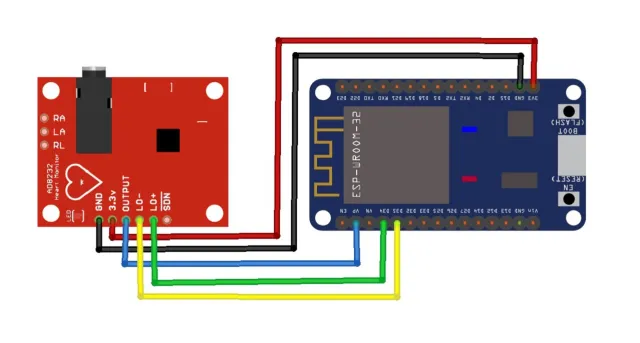
\includegraphics[scale=.4]{imgs/AD8232ESP32.png}
  \caption{Interfaçage du capteur AD8232 avec la carte de développement ESP32}
\end{figure}

Pour que le système soit en marche, il faut ajouter :
\begin{enumerate}
  \item une connexion INTERNET : la carte ESP32 peut se connecter à un réseau WIFI. Mais un tel réseau doit assurer une connexion à INTERNET et n'est pas un simple réseau local par exemple.
  \item un serveur de données : il faut avoir un accès à un serveur dans le WEB afin d'y enregistrer les informations récupérées du capteur. Ainsi, une inscription dans une plateforme dédiée peut donner ce type d'accès.
\end{enumerate}

Jusqu'à présent, la partie hardware du projet a été investiguée. En se basant sur cette architecture, quels sont les composants software à ajouter permettant le bon fonctionnement du système ?
\section{Composante logicielle}
  \appendix
  \chapter{Datasheet du capteur AD8232\label{Datasheet}}
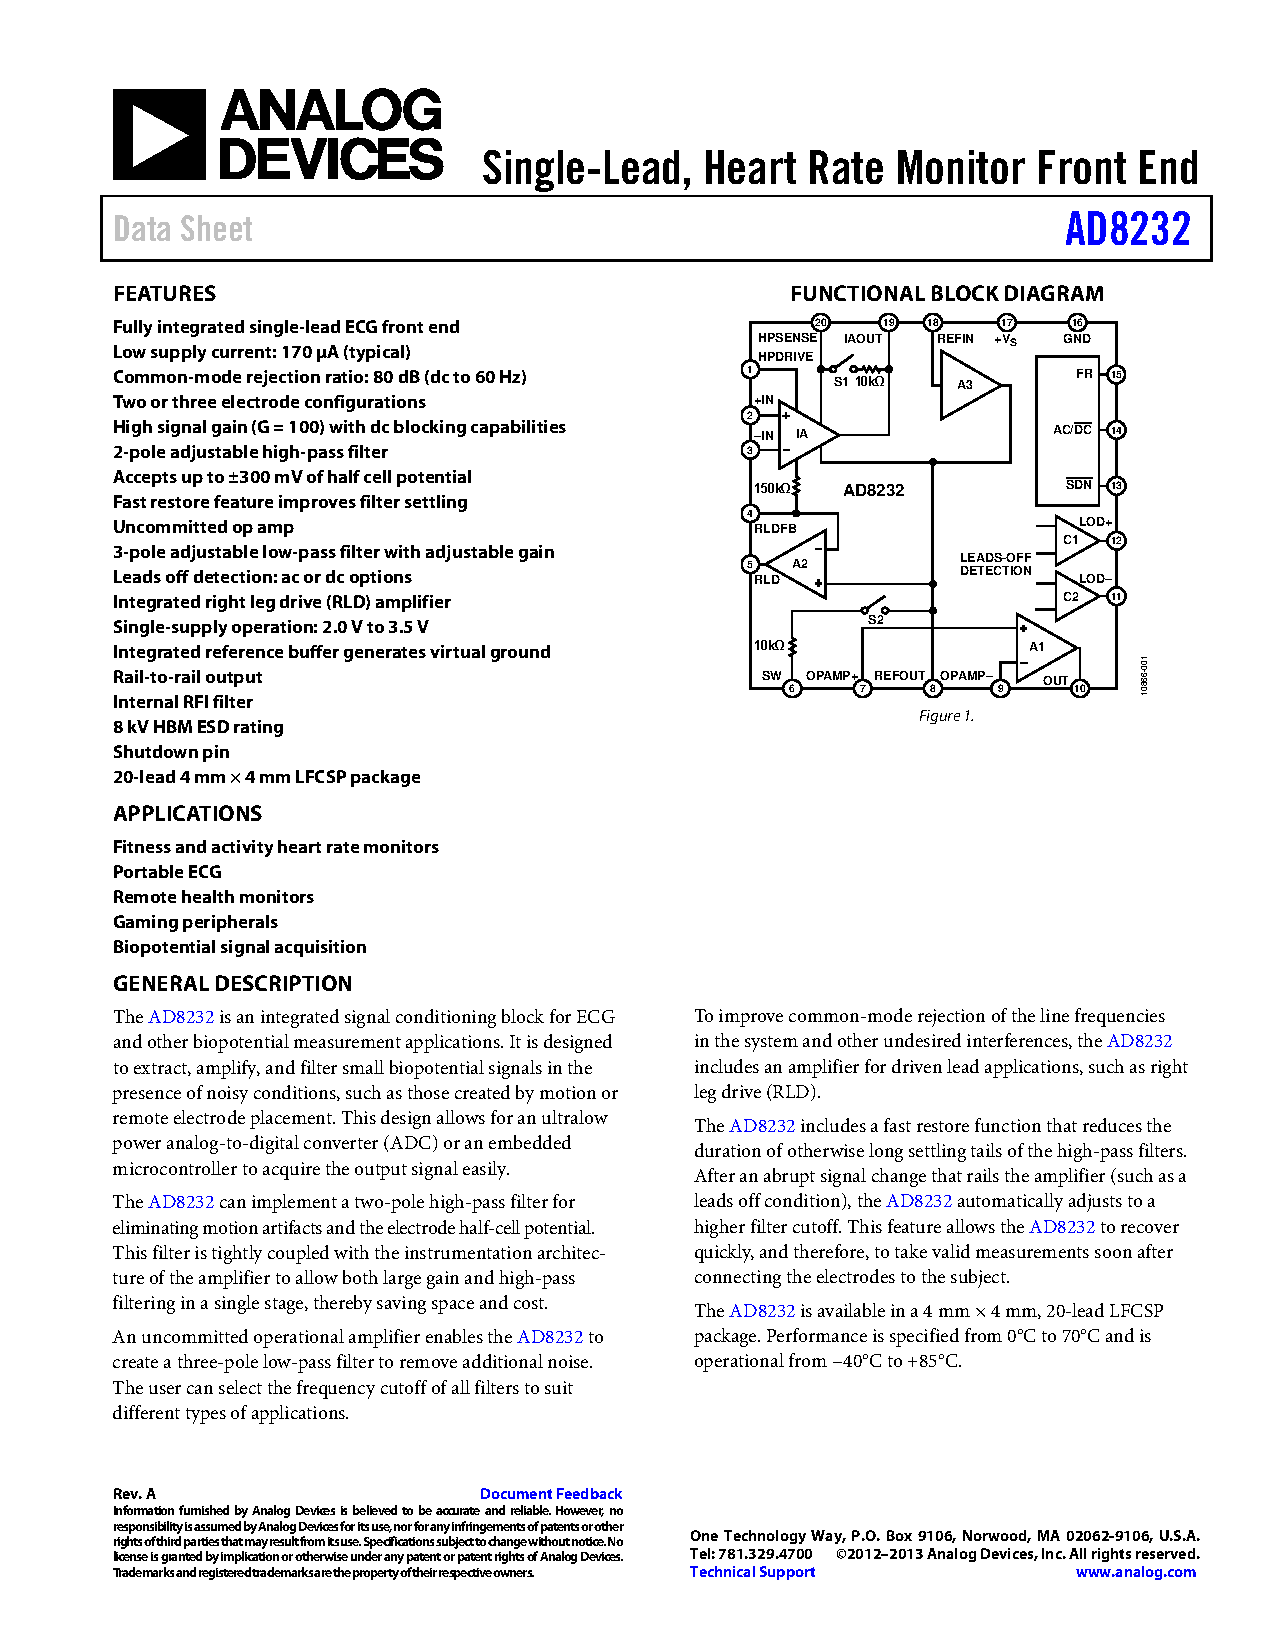
\includepdf[pages={1,3,4,5}]{Docs/AD8232.PDF}
  \section{Code source\label{codesource}}
\begin{mycpp}
  /**
* @file main.cpp
* @author N. AZZOUZ, A. MELLAH, R. ALOUI
* @brief 
* @version 0.1
* @date 2023-01-14
* 
* @copyright Copyright (c) 2023
* 
*/
#include <Arduino.h>

#include <WiFi.h>
#include <WiFiUdp.h>  // Utilisation du protocole UDP (pour les applications temps réel)
#include <PubSubClient.h>
#include <NTPClient.h>


#define WIFISSID "Redmi Note 11" // Enter WifiSSID here
#define PASSWORD "isetbeja" // Enter password here
#define TOKEN "BBFF-Hz6tdZJl9805kiV1KRrxKrXaEjIV24" // Ubidots' TOKEN
#define MQTT_CLIENT_NAME "BBFF-Hz6tdZJl9805kiV1KRrxKrXaEjIV24" // MQTT client Name
#define VARIABLE_LABEL "ecg_val" // ubidots variable label
#define DEVICE_LABEL "AD8232_IASRIA" // ubidots device label
#define T_SAMPLING 150 // Period of sampling (ms)


#define SENSORPIN A0 // Set the A0 as SENSORPIN

char mqttBroker[]  = "industrial.api.ubidots.com";
char payload[10000];
char topic[150];
// Space to store values to send
char str_sensor[10];
char str_millis[20];
double epochseconds = 0;
double epochmilliseconds = 0;
double current_millis = 0;
double current_millis_at_sensordata = 0;
double timestampp = 0;
int j = 0;
/****************************************
 Auxiliar Functions
****************************************/
WiFiClient ubidots;
PubSubClient client(ubidots);
WiFiUDP ntpUDP;
NTPClient timeClient(ntpUDP, "pool.ntp.org");

void callback(char* topic, byte* payload, unsigned int length) {
char p[length + 1];
memcpy(p, payload, length);
p[length] = NULL;
Serial.write(payload, length);
Serial.println(topic);
}

void reconnect() {
// Loop until we're reconnected
while (!client.connected()) {
  Serial.println("Attempting MQTT connection...");

  // Attemp to connect
  if (client.connect(MQTT_CLIENT_NAME, TOKEN, "")) {
    Serial.println("Connected");
  } else {
    Serial.print("Failed, rc=");
    Serial.print(client.state());
    Serial.println(" try again in 2 seconds");
    // Wait 2 seconds before retrying
    delay(2000);
  }
}
}

/****************************************
 setup function
****************************************/
void setup() {
Serial.begin(115200);
WiFi.begin(WIFISSID, PASSWORD);
// Assign the pin as INPUT
pinMode(SENSORPIN, INPUT);

Serial.println();
Serial.print("Waiting for WiFi...");

while (WiFi.status() != WL_CONNECTED) { // Try to connect to network
  Serial.print(".");
  delay(500);
}

Serial.println("");
Serial.println("WiFi Connected");
Serial.println("IP address: ");
Serial.println(WiFi.localIP());
timeClient.begin();
client.setServer(mqttBroker, 1883); // Try to connect to MQTT server
client.setCallback(callback);
timeClient.update();
epochseconds = timeClient.getEpochTime();
epochmilliseconds = epochseconds * 1000;
Serial.print("epochmilliseconds=");
Serial.println(epochmilliseconds);
current_millis = millis();
Serial.print("current_millis=");
Serial.println(current_millis);
}

/****************************************
 setup function
****************************************/
void loop() {
if (!client.connected()) {
  reconnect();
  j = 0;
}

j = j + 1;  // Messages sent
Serial.print("j=");
Serial.println(j);
sprintf(topic, "%s%s", "/v1.6/devices/", DEVICE_LABEL);
sprintf(payload, "%s", ""); // Cleans the payload
sprintf(payload, "{\"%s\": [", VARIABLE_LABEL); // Adds the variable label
for (int i = 1; i <= 3; i++)
{
  float sensor = analogRead(SENSORPIN); // Read from sensor
  dtostrf(sensor, 4, 2, str_sensor);
  sprintf(payload, "%s{\"value\":", payload); // Adds the value
  sprintf(payload, "%s %s,", payload, str_sensor); // Adds the value
  current_millis_at_sensordata = millis();
  timestampp = epochmilliseconds + (current_millis_at_sensordata - current_millis);
  dtostrf(timestampp, 10, 0, str_millis);
  sprintf(payload, "%s \"timestamp\": %s},", payload, str_millis); // Adds the value
  delay(T_SAMPLING);
}

float sensor = analogRead(SENSORPIN); // Read from sensor
dtostrf(sensor, 4, 2, str_sensor);
current_millis_at_sensordata = millis();
timestampp = epochmilliseconds + (current_millis_at_sensordata - current_millis);
dtostrf(timestampp, 10, 0, str_millis);
sprintf(payload, "%s{\"value\":%s, \"timestamp\": %s}]}", payload, str_sensor, str_millis);
Serial.println("Publishing data to Ubidots Cloud");
client.publish(topic, payload); // Publish data to ubidots.com
Serial.println(payload);
delay(T_SAMPLING);
}
  \end{mycpp}
  \section{Output\label{output}}

\begin{commandshell}
  Waiting for WiFi.........
WiFi Connected
IP address:
192.168.1.6
epochmilliseconds=ovf
current_millis=3362.00
Attempting MQTT connection...
Connected
j=1
Publishing data to Ubidots Cloud
{"ecg_val": [{"value": 4095.00, "timestamp": 1673654680417},{"value": 4095.00, "timestamp": 1673654680567},{"value": 4095.00, "timestamp": 1673654680717},{"value":4095.00, "timestamp": 1673654680867}]}
j=2
Publishing data to Ubidots Cloud
{"ecg_val": [{"value": 4095.00, "timestamp": 1673654680878},{"value": 4095.00, "timestamp": 1673654681029},{"value": 4095.00, "timestamp": 1673654681179},{"value":4095.00, "timestamp": 1673654681329}]}
j=3
Publishing data to Ubidots Cloud
{"ecg_val": [{"value": 4095.00, "timestamp": 1673654681339},{"value": 4095.00, "timestamp": 1673654681489},{"value": 4095.00, "timestamp": 1673654681639},{"value":4095.00, "timestamp": 1673654681789}]}
j=4
Publishing data to Ubidots Cloud
{"ecg_val": [{"value": 4095.00, "timestamp": 1673654681800},{"value": 4095.00, "timestamp": 1673654681950},{"value": 4095.00, "timestamp": 1673654682100},{"value":4095.00, "timestamp": 1673654682250}]}
j=5
Publishing data to Ubidots Cloud
{"ecg_val": [{"value": 4095.00, "timestamp": 1673654682260},{"value": 4095.00, "timestamp": 1673654682410},{"value": 4095.00, "timestamp": 1673654682560},{"value":4095.00, "timestamp": 1673654682710}]}
j=6
Publishing data to Ubidots Cloud
{"ecg_val": [{"value": 4095.00, "timestamp": 1673654682721},{"value": 4095.00, "timestamp": 1673654682871},{"value": 4095.00, "timestamp": 1673654683021},{"value":4095.00, "timestamp": 1673654683171}]}
j=7
Publishing data to Ubidots Cloud
{"ecg_val": [{"value": 4095.00, "timestamp": 1673654683181},{"value": 4095.00, "timestamp": 1673654683331},{"value": 4095.00, "timestamp": 1673654683481},{"value":4095.00, "timestamp": 1673654683631}]}
j=8
Publishing data to Ubidots Cloud
{"ecg_val": [{"value": 4095.00, "timestamp": 1673654683642},{"value": 4095.00, "timestamp": 1673654683793},{"value": 4095.00, "timestamp": 1673654683943},{"value":4095.00, "timestamp": 1673654684093}]}
j=9
Publishing data to Ubidots Cloud
{"ecg_val": [{"value": 4095.00, "timestamp": 1673654684103},{"value": 4095.00, "timestamp": 1673654684253},{"value": 4095.00, "timestamp": 1673654684403},{"value":4095.00, "timestamp": 1673654684553}]}
j=10
Publishing data to Ubidots Cloud
{"ecg_val": [{"value": 4095.00, "timestamp": 1673654684564},{"value": 4095.00, "timestamp": 1673654684715},{"value": 4095.00, "timestamp": 1673654684865},{"value":4095.00, "timestamp": 1673654685015}]}
j=11
Publishing data to Ubidots Cloud
{"ecg_val": [{"value": 4095.00, "timestamp": 1673654685025},{"value": 4095.00, "timestamp": 1673654685176},{"value": 4095.00, "timestamp": 1673654685326},{"value":4095.00, "timestamp": 1673654685476}]}
j=12
Publishing data to Ubidots Cloud
{"ecg_val": [{"value": 4095.00, "timestamp": 1673654685487},{"value": 4095.00, "timestamp": 1673654685638},{"value": 4095.00, "timestamp": 1673654685788},{"value":4095.00, "timestamp": 1673654685938}]}
\end{commandshell}
  %\chapter{Conception}
  %\section{Mise en cadre du projet}
  %\chapter{Réalisation}
  \bibliographystyle{plain}
  \bibliography{Bibs/mybib.bib}
\end{document}